\section{Efficient Semantic Parsing}
\label{sec:parsing}
In this section we explain our algorithms and heuristics for efficient semantic
parsing with as little non-determinism as possible, and reducing time complexity
of our parsing strategies.

\subsection{Naïve Semantic Parsing on Syntactic Parsing}
In this section we suppose that we have a set of syntax trees
(or parsing trees) corresponding to a certain sentence.
We will now focus on how to derive proofs of typing from a syntax tree.
First, note that \cite{bumfordEffectdrivenInterpretationFunctors2025} provides
a way to do so by constructing semantic trees labelled by sequence of
\emph{combinators} (see Section \ref{subsec:ssparsing}).
In our formalism, this amounts to constructing proof trees by mapping
combination modes to their equivalent proof trees, inverting if needed the
order of the presuppositions to account for the order of the words.
Computing one tree is easily done in linear time in the number of nodes in the
parsing tree (which is linear in the input size, more on that in the next
section), multiplied by a constant whose size depends on the size of the
inference structure.
The main idea is that to each node of the tree, both nodes have a type and
there is only a finite set of rules that can be applied, provided by the
following rules, which are a rewriting of Figure \ref{tab:judgements}.
In Figure \ref{tab:proof-trees} we provide \emph{matching-like} rules for
different possibilities on the types to combine and the associated possible
proof tree(s).
Note that there is no condition on what the types \emph{look like}, they can
be effectful.
If multiple cases are possible, all different possible proof trees should be
added to the set of derivations: the set of proof trees for the union of cases
is the union of set of proof trees for each case, naturally.

\begin{figure*}
	\centering
	\inputtikz{match-judgement}
	\caption{List of possible combinations for different presuppositions for inputs, as a definition of a function
		$PT$ from proof trees to proof trees.}
	\label{tab:proof-trees}
\end{figure*}

This leads the induced algorithm (for computing the set of denotations) to be
exponential in the input in the worst case, when using the recursive scheme
that naturally arises from the definition of $PT$.
Indeed, and while this may seem weird, in the case of a function
$\f{F}\ta \to \tb$ where $\f{F}$ is applicative and the other combinator is of
type $\f{F}\ta$, one might apply the function directly or apply it under the
$\f{F}$ of the argument, leading to two different proof trees:
\begin{align*}
	\columneqs{\prooffrac{\cont \f{F}: \mC \Rightarrow \mC \poulpe \Junit{\f{F}}{l}{\ta}{r}{\tb}}{\cont \f{F}lr: \f{F}\tb}} \\[1em]
	\Japp{l}{\f{F}\ta}{\tb}{r}
\end{align*}
Those two different proof trees have different semantic interpretations that
may be useful, as discussed by
\cite{bumfordEffectdrivenInterpretationFunctors2025}, especially in their
analysis of closure properties, which is modified in the following section.

\subsubsection{Islands}
\cite{bumfordEffectdrivenInterpretationFunctors2025} provide a formal analysis
of islands\footnote{Syntactic structures which prevent some notion of moving
	outside of the island.} based on a islands being a different type of branching
nodes in the syntactic tree of a sentence, which asks to resolve all $\f{C}$
effects\footnote{Those represent quantifications.} before that node or being
resolved at that node.

To reconcile this inside our type system, we propose the following change to
their formalism: once the syntactic information of an island existing is added
to the tree, we \emph{mark} each node inside the island by adding a ``void
effect'' to it, in the same way as we did for our model of plural.
This translates into a functor which just maintains the \emph{island marker} on
\texttt{fmap} and change the type of the boundary word to one that cannot take
a continuation as input, which could be seen as adding a node in the semantics
parse tree from the syntactic parse tree.
A way to do this would be the following: we pass all functors until finding a
$\f{C}$, handle it inside the other functors and keep going, on both sides,
where $\mathrm{PT}$ is defined in Figure \ref{tab:proof-trees}:
\begin{equation*}
	\mathrm{PT}\left(
	\suppfrac{\raisebox{-5pt}{$\cont x_{1}: \f{F}\f{C}\f{F'}\tau$}}{\cont x_{1}: \f{F}\f{F'}\tau}\suchthat
	\suppfrac{\raisebox{-5pt}{$\cont x_{2}: \f{F}\f{C}\f{F'}\tau$}}{\cont x_{2}: \f{F}\f{F'}\tau}
	\right)
\end{equation*}
Note that this preserves the linear size of the parse tree in the number of
input words, as we at most double the number of nodes, and note that this
would be preserved with additional similar constructs.

\medskip

This idea amounts to seeing islands, whatever their type, as a form of
grammatical/syntactic effect, which is still part of the language but not of
the lexicon, a bit like future, modality or plurals, without the semantic
component.
The idea of seeing everything as effects, while semantically void, allows us
to translate into our theory of type-driven semantics outer information from
syntax, morphology or phonology that influences the semantics of the
sentence, and make use of the type system to enforce them.
Other examples of this can be found in the modelisation of plural (for
morphology, see Sections \ref{par:higherorder} and \ref{subsec:modality})
and the emphasis of the words by the $\f{F}$ effect (for phonology), and show
the empirical well-foundedness of this point of view.
While we do not aim to provide a theory of everything linguistics through
categories, the idea of expressing everything in our effect-driven type-driven
theory of semantics allows us to prepare for any theoretical or empirical
observation that has an impact on the semantics of a word/sentence, the allowed
combinators and even the addition of rules.

\subsection{Syntactic-Semantic Parsing}
\label{subsec:ssparsing}
\subsubsection{The Improved Method}
As using a naïve strategy on the trees yields an exponential algorithm,
we will simply extend the grammar system used to do the syntactic part of the
parsing.
In this section, we will take the example of a CFG since it suffices to create
our typing combinators.
Here, we change our notations from the proof trees of Figure
\ref{tab:proof-trees} to have a more explicit grammar of combination modes
provided below is a rewriting of the proof trees provided earlier, and
highlights the combination modes in a simpler way, based on
\cite{bumfordEffectdrivenInterpretationFunctors2025} as it simplifies the
rewriting of our typing judgements in a CFG.
The grammars provided in Figures \ref{fig:english-cfg} and
\ref{fig:combination-cfg} are the ones used in the parsing.

\begin{figure}
	\centering
	\inputtikz{combination-cfg}
	\caption{Possible Type Combinations in the form of a near CFG}
	\label{fig:combination-cfg}
\end{figure}

The grammar in Figure \ref{fig:combination-cfg} works in five major sections:
\begin{enumerate}
	\item We reintroduce the grammar defining the type and effect system.
	\item We introduce a structure for the semantic parse trees and their labels,
	      the combination modes from
	      \cite{bumfordEffectdrivenInterpretationFunctors2025}.
	\item We introduce rules for basic type combinations.
	\item We introduce rules for higher-order unary type combinators.
	\item We introduce rules for higher-order binary type combinators.
\end{enumerate}
We do not prove here that these typing rules cannot be written in a simpler
syntactic structure.

\medskip

The idea of the \emph{grammatical} reduction is that from two words that can
syntactically combine, we use the binary effect combinators, before choosing
the appropriate binary type combinator.
It is at this point in the reduction we actually do the compositional part.
We close up the reduction by possibly using unary effect combinators.
This work is done for combinators of arity two, but could be extended, as seen
in Appendix \ref{app:arities-and-denots}.

For example, the rules of the form $\combML_{\f{F}} M, \tau' \gets M, \tau$ are
rules that provide ways to combine effects from the two inputs in the order we
want to: we can combine $\f{R}\f{S}\e$ and $\f{C}\f{W}(\e \to \t)$ into
$\f{R}\f{C}\f{W}\f{S}\t$ with the mode $\combML\combMR\combMR\combML <$ (see
\cite{bumfordEffectdrivenInterpretationFunctors2025} Example 5.14).

\begin{figure}
	\centering
	\inputtikz{combinator-denotations}
	\caption{Denotations describing the effect of the combinators used in the
		grammar describing our combination modes presented in
		Figure \ref{fig:combination-cfg}}
	\label{fig:combinator-denotations}
\end{figure}

Each of these combinators can be, up to order, associated with a inference
rule, and, as such, with a higher-order denotation, which explains the actual
effect of the combinator, and are described in Figure
\ref{fig:combinator-denotations}.
The main reason we need to get denotations associated to combinators, is to
properly define the combination of words/phrases that underlines our system.
The important thing on those denotations is that they're a direct translation
of the rules defining the notions of functors, applicatives, monads and thus
are not specific to any denotation system, even though we will use
lambda-calculus styled denotations to describe them.
This makes us able to compute the actual denotations associated to a sentence
using our formalism, as presented in figure \ref{fig:parsing-trees}.
Note that the order of combination modes is not actually the same as the one
that would come from the grammar.
The reason why will become more apparent when string diagrams for parsing are
introduced in the next section, but simply, this comes from the fact that while
we think of $\combML$ and $\combMR$ as reducing the number of effects on each
side (and this is the correct way to think about those), this is not actually
how their denotations work, for simplicity of writing the denotations, and
simplicity of doing the parsing.

\begin{figure}
	\centering
	\begin{subfigure}{.9\columnwidth}
	\centering
	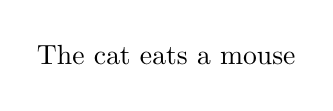
\begin{tikzpicture}[every node/.style={align=center, minimum height=2em, minimum width=1cm}]
		\Tree [ .\node{The cat eats a mouse}; {A} {B} ]
	\end{tikzpicture}
	\caption{Labelled tree representing the equivalent parsing diagram to
		\ref{fig:parsing-diagram}}
\end{subfigure}

\medskip

\begin{subfigure}{.9\columnwidth}
	\centering
	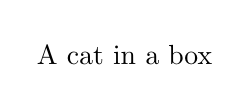
\begin{tikzpicture}[every node/.style={align=center, minimum height=2em, minimum width=1cm}]
		\Tree [ .\node{A cat in a box}; {C} {D} ]
	\end{tikzpicture}
	\caption{Labelled tree representing the equivalent parsing diagram to
		\ref{fig:parsing-diagram2}}
\end{subfigure}

\medskip

\begin{subfigure}{.9\columnwidth}
	\centering
	\begin{tikzpicture}[every node/.style={align=center, inner sep=6pt}, level distance=1.5cm]
		\Tree [
		.\node[comb={$>$}]{\t \\ $\mathbf{if}(\forall x. \w{pass} x)\w{rain}$};
		[ .\node[comb={$>$}]{$\t \to \t$ \\ $\mathbf{if}(\forall x.\w{pass} x)$};
		{$\t \to \t \to \t$ \\ if}
		[
		.\node{$\t$\\ $\forall x. \w{pass} x$ \\ $\combDN_{\Downarrow_{\f{C}}}$};
		[ .\node[comb={$\combMR_{\f{C}}<$}]{$\f{C}\t$ \\ $\lambda c.\forall x. c(\w{pass} x)$};
		{$\f{C}\e$ \\ $\lambda c. \forall x. c\, x$ \\ everyone}
		{$\e \to \t$ \\ $\mathbf{pass}$ \\ passed}
		]
		]
		]
		[
		.{\t \\ $\mathbf{rain}$} \edge[roof]; {it was raining}
		]
		]
	\end{tikzpicture}
	\caption{Labelled tree representing the equivalent parsing diagram to
		\ref{fig:3dparsing-diagram}}
\end{subfigure}

	\caption{Examples of Labeled Parse Trees for a few sentences.}
	\label{fig:parsing-trees}
\end{figure}

\medskip

Since our grammar is defined with respect to the functor set, the algorithm
which parses the combinators will have a complexity in the size of
$\mFunc\left(\mL\right)$ that is linear, which comes from the fact that our
grammar's size is linear in $\abs{\mFunc\left(\mL\right)}$.

\begin{thm}
	\label{thm:ptime-parse}
	Semantic parsing of a sentence is polynomial in the length of the	sentence
	and the size of the type system and syntax system.
\end{thm}
\begin{proof}
	Suppose we are given a syntactic generating structure $G_{s}$ along with our
	type combination grammar $G_{\tau}$.
	The system $G$ that can be constructed from the (tensor) product of $G_{s}$ and
	$G_{\tau}$ has size $\abs{G_{s}}\times \abs{G_{\tau}}$.
	Indeed, we think of its rules as a rule for the syntactic categories and a rule
	for the type combinations. Its terminals and non terminals are also in the
	cartesian products of the adequate sets in the original grammars.
	What this in turn means, is that if we can syntactically parse a sentence in
	polynomial time in the size of the input and in $\abs{G_{s}}$, then we can
	syntactico-semantically parse it in polynomial time in the size of the input,
	$\abs{G_{s}}$ and $\abs{G_{\tau}}$.
\end{proof}

While we have gone with the hypothesis that we have a CFG for our language,
any type of polynomial-time structure could work, as long as it is as
expressive as a CFG.
We will do the following analysis using a CFG since it allows to cover enough
of the language for our example and for simplicity of describing the process of
adding the typing CFG, even though some think that English is not a context
free language \cite{higginbothamEnglishNotContextFree1984}.

\begin{thm}
	\label{thm:ptime-denot}
	Retrieving a pure denotation for a sentence can be done in polynomial time in
	the length of the sentence, given a polynomial time syntactic parsing
	algorithm and polynomial time combinators.
\end{thm}
\begin{proof}
	We have proved in Theorem \ref{thm:ptime-parse} that we can retrieve a
	semantic parse tree from a	sentence in polynomial time in the input.
	Since we also have shown that the length of a semantic parse tree is quadratic
	in the length of the sentence it represents, being linear in the length of a
	syntactic parse tree linear in the length of the sentence.
	We have already seen that given a denotation, handling all effects and
	reducing effect handling to normal forms can be done in polynomial time.
	The superposition of these steps yields a polynomial-time algorithm in the
	length of the input sentence.
\end{proof}

The \emph{polynomial time combinators} assumption is not a complex assumption,
this is for example true for our denotations in Section \ref{sec:language},
with function application being linear in the number of uses of variables in
the function term, which in turn is linear in the number of terms used to
construct the function term and thus of words, and \fmap being in constant
time\footnote{Depending on the functor but still bounded by a constant.} for
the same reason.

\subsubsection{Diagrammatical Parsing}
\label{subsubsec:diagram-parsing}
When considering \cite{coeckeMathematicalFoundationsCompositional2010}
way of using string diagrams for syntactic parsing/reductions, we can see them
as (yet) another way of writing our parsing rules.
In our typed category, we can see our combinators as natural
transformations ($2$-cells): then we can see the different sets of combinators
as different arity natural transformations.
$>$, $\combML_{\f{F}}$ and $\combJ_{\f{F}}$ are represented in
Figure \ref{fig:combinator-sd}, up to the coloring of the regions, because that
is purely for an artistic rendition.

\begin{figure}
	\centering
	\inputtikz{combinators-sd}
	\caption{String Diagramatic Representation of Combinator Modes $>, \combML$ and $\combJ$}
	\label{fig:combinator-sd}
\end{figure}

Now, a way to see this would be to think of this as an orthogonal set of
diagrams to the ones of Section \ref{sec:nondet}: we can use the syntactic
version of the diagrams to model our parsing, according to the rules in
Figure \ref{fig:combination-cfg}, and then combine the diagrams as shown in
Figure \ref{fig:parsing-diagram}.
This explains the construction of the diagrams in Section \ref{sec:nondet}.
In this figure we exactly see the sequence of reductions play out on the types
of the words, and thus we also see what exact \emph{quasi-braiding} would be
needed to construct the effect diagram.
Here we talk about \emph{quasi-braiding} because, in a sense, we use $2$-cells
to do braiding-like operations on the strings, and don't actually allow for
braiding inside the diagrammatic calculus.
To better understand what happens in those parsing diagrams, Figure
\ref{fig:parsing-trees} provides the translations in labelled trees of the
parsing diagrams of Figures \ref{fig:parsing-diagram},
\ref{fig:parsing-diagram2} and \ref{fig:3dparsing-diagram}.


\begin{figure}
	\centering
	\inputtikz{parsing-diagram}
	\caption{Representation of a parsing diagram for the sentence
		\emph{the cat eats a mouse}.
		See Figure \ref{fig:tree-box} for translation in a parse tree.}
	\label{fig:parsing-diagram}
\end{figure}

Categorically, what this means is that we start from a meaning category $\mC$,
our typing category, and take it as our grammatical category.
This is a form of extension on the monoidal version by
\cite{coeckeMathematicalFoundationsCompositional2010}, as it is seemingly a
typed version, where we change the Pregroup category for the typing category,
possibly taken with a product for representation of the English grammar
representation, to accomodate for syntactic typing on top of semantic typing.
This is, again, just another rewriting of our typing rules.

We have a first axis of string diagrams in the category
$\mC$ - our string diagrams for effect handling, as in Section
\ref{sec:nondet} - and a second \emph{orthogonal} axis of string diagrams
on a larger category, with endofunctors graded by the types in our typing
category $\bar{\mC}$ and with natural transformations mapping the combinators
defined in Figures \ref{fig:combination-cfg} and
\ref{fig:combinator-denotations}.
The category in which we consider the second-axis string diagrams does not have
a meaning in our compositional semantics theory, and to be more precise, we
should talk about $1$-cells and $2$-cells instead of functors and natural
transformations, to keep in the idea that this is really just a diagrammatic
way of computing and presenting the operations that are put to work during
semantic parsing.

\medskip

What the lines leading from combinators to functors mean categorically, is
void in either category.
Those lines are not actually part of the first axis of the string diagram,
nor are they part of the second axis of the string diagram.
They are used to map out the link between the two: they express the
quasi-braiding step proposed above, and present graphically why the order of
the strings in the resulting diagram is as it is, and what the pasting and
quasi-braiding orders should be.
These diagrams are an extension of the parse trees presented in
\cite{bumfordEffectdrivenInterpretationFunctors2025} in a graphical format and
extended to be integrated with the handling of effects, as described in Section
\ref{sec:nondet}, forming a full diagrammatic calculus system for semantic
parsing.

\medskip

Applying the unary combinators which reduce effects to the actual
\emph{parsing} part of the diagram is done in the exact same way as in the CFG,
we just apply them when needed, and they will appear in the resulting
denotation as an end for a string, a form of forced handling, in a sense, as
shown in the result of Figure \ref{fig:parsing-diagram2}.
For the connecting strings, it's simply a matter of adding a new \emph{phantom}
string that will send the associated $2$-cell in the effect handling diagram to
the connected strings.
In particular it is interesting to note that the resulting diagram representing
the sentence can, in a way, be found in the connection strings that arise from
the combinators, which justifies again the shape of the diagrams in Section
\ref{sec:nondet}.

\begin{figure}
	\centering
	\inputtikz{parsing-diagram2}
	\caption{Example of a parsing diagram for the phrase
		\emph{a cat in a box}, presenting the integration of unary combinators
		inside the connector line.
		See Figure \ref{fig:tree-box} for translation in a parse tree.}
	\label{fig:parsing-diagram2}
\end{figure}

One of the main reasons why this point of view of diagrammatic parsing is
useful will be clear when looking at the rewriting rules and the normal forms
they induce, because, as seen before, string diagrams make it easy to compute
normal forms, when provided with a confluent reduction system.

\begin{figure}
	\centering
	\begin{tikzpicture}
		\node (fig) at (0, 0)
		{\includegraphics[width=.8\columnwidth]{aux/figures/knitting-example}};
		\draw[->] ($(fig.south west) + (-.1, -.1)$) -- node[anchor=east]
		{\rotatebox{90}{Direction of Reduction}} ($(fig.north west) + (-.1, .1)$);
	\end{tikzpicture}
	\caption{Example of a \emph{Jacquard} knitwork.
		Photography and work courtesy of the author's mother.}
	\label{fig:knitting-example}
\end{figure}

The other reason being the tangible interpretation of how things work
underlying the idea of a string diagram:
Suppose you're knitting a rainbow scarf.
You have multiple threads (the different words) of the different colours (their
types and effects) you're using to knit the scarf.
When you decide to change the color you take the different threads you have
been using, and mix them up:
You can create a new colour\footnote{I know this is not how wool works, but
	if you prefer you can imagine a pointillist-like way of drawing using multiple
	coloured lines that superimpose on each other, or a marching band's multiple
	instruments playing either in harmony or in disharmony and changing that
	during a score.} thread from two (that's the base combinators) create a
thicker one from two of the same colour (the applicative mode and the monadic
join), put aside a thread until a later step (that's the $\fmap$), add a new
thread to the pattern (that's the unit), or cut a thread you will not be
using anymore (that's the co-units and closure operators).
Changing a thread by cutting it and making a knot at another point is basically
what the eject combinators do.
This more tangible representation can be seen in a larger diagram in Figure
\ref{fig:3dparsing-diagram}.
The sections in the rectangle represent what happen when considering our
combination step as implementing patterns inside a knitwork, as seen in Figure
\ref{fig:knitting-example}.
The different patterns provide, in order, a visual representation of the
different ways one can combine two strings, i.e., two types and thus two
denotations.
The sections outside of the rectangle are the strings of yarn not currently
being used to make a pattern.

\begin{figure*}
	\centering
	\begin{tikzpicture}
	\path
	(0, 0) coordinate[label=$\t \to \t \to \t$] (t1)
	++ (1.5, 0) coordinate[label=$\f{C}$] (tf2)
	+ (.5, 0) coordinate[label=$\e$] (tt2)
	++ (1, 0) coordinate[label=$\e\to\t$] (t3)
	++ (1, 0) coordinate[label=$\t$] (t4);
\end{tikzpicture}

	\caption{3D-like Representation of the Diagrammatic Parsing of a Sentence. See \ref{fig:tree-rain} for the translation in a Parse Tree}
	\label{fig:3dparsing-diagram}
\end{figure*}

\subsection{Rewriting Rules}
\label{subsec:rewrite}
Here we provide a rewriting system on derivation trees that allows us to
improve our time complexity by reducing the size of the disambigued grammar.
In the worst case, in big o notation there is no improvement in the size of the
sentence, but there is no loss.

\medskip

First, let's consider the reductions proposed in Section \ref{sec:nondet}.
Those define normal forms under Theorem \ref{thm:confluence} and thus we can
use those to reduce the number of trees.
Indeed, we usually want to reduce the number of effects by first using the
rules \emph{inside} the language, understand, the adjunction co-unit and
monadic join.
This in turn means we always verify the derivational rules we set up in the
previous section for the join equations of the monad.

\medskip

Secondly, while there is no way to reduce the branching proposed in the
previous section since they end in completely different reductions, there is
another case in which two different reductions arise:
\begin{equation*}
	\PT{\blank}{\cont x: \f{F}\tau_{1}} \poulpe \text{and} \poulpe
	\PT{\blank}{\cont y: \f{G}\tau_{2}}
\end{equation*}
Indeed, in that case we could either get a result with effects $\f{F}\f{G}$ or
with effects $\f{G}\f{F}$.
In general those effects are not the same, but if they happen to be, which
trivially will be the case when one of the effects is external, the plural or
islands functors for example.
When the two functors commute, the order of application does not matter and
thus we choose to get the outer effect the one of the left side of the
combinator.

\medskip

Thirdly, there are modes that clearly encompass other ones.
One should not use mode $\combUR$ when using $\combMR$ or $\combDN \combMR$
and the same goes for the left side, because the two derivations yield simpler
results.
Same things can be said for certain other derivations containing the lowering
and co-unit combinators.

\noindent We use $\combDN$ when we have not used any of the following, in all
derivations:
\begin{multicols}{2}
	\begin{itemize}
		\item $m_{\f{F}}, \combDN, m_{\f{F}}$ where
		      $m \in \{\combMR, \combML\}$
		\item $\combML_{\f{F}}, \combDN, \combMR_{\f{F}}$
		\item $\combA_{\f{F}}, \combDN, \combMR_{\f{F}}$
		\item $\combML_{\f{F}}, \combDN, \combA_{\f{F}}$
		\item $\combC$
	\end{itemize}
\end{multicols}
\noindent We use $\combJ$ if we have not used any of the following,
for $j \in \{\epsilon, \combJ_{\f{F}}\}$
\begin{multicols}{2}
	\begin{itemize}
		\item $\left\{m_{\f{F}}, j, m_{\f{F}}\right\}$ where
		      $m \in \{\combMR, \combML\}$
		\item $\combML_{\f{F}}, j, \combMR_{\f{f}}$
		\item $\combA_{\f{F}}, j, \combMR_{\f{F}}$,
		\item $\combML_{\f{F}}, j, \combA_{\f{F}}$
		\item $k, \combC$ for $k \in \{\epsilon, \combA_{\f{F}}\}$
		\item If $\f{F}$ is commutative as a monad:
		      \begin{itemize}
			      \item $\combMR_{\f{F}}, \combA_{\f{F}}$
			      \item $\combA_{\f{F}}, \combML_{\f{F}}$
			      \item $\combMR_{\f{F}}, j, \combML_{\f{F}}$
			      \item $\combA_{\f{F}}, j, \combA_{\f{F}}$
		      \end{itemize}
	\end{itemize}
\end{multicols}
Similar facts can be given for the co-units of an adjunction.

\begin{thm}
	The rules proposed above yield equivalent results.
\end{thm}
\begin{proof}
	For the first point, the equivalence has already been proved under Theorem
	\ref{thm:confluence}.
	For the second point, it is obvious since based on an equality.
	For the third point, it's a bit more complicated.
	The rules about not using combinators $\combUL$ and $\combUR$ come from the
	notion of handling and granting termination and decidability to our system.
	The rules about adding $\combJ$ and $\combDN$ after moving two of the same
	effect from the same side (i.e. $\combML \combML$ or $\combMR\combMR$) are
	normalization of a the elevator equations \ref{eq:elevator}.
	Indeed, in the denotation, the only reason to keep two of the same effects
	and not join them\footnote{Provided they can be joined.} is to at some point
	have something get in between the two.
	Joining and cloture should then be done at earliest point in parsing where it
	can be done, and that is equivalent to later points because of the elevator
	equations, or Theorem \ref{thm:isotopy}.
	The last set of rules follows from the following: we should not use $\combJ
		\combML \combMR$ instead of $\combA$, as those are equivalent because of the
	equation defining them.
	The same thing goes for the other facts, as we should use the units of monads
	over applicative rules and fmap.
\end{proof}

This is simply a scheme to apply typing rules to a syntactic derivation,
but that this will not be enough to actually gain all reductions possible
in polynomial time.
This is actually not feasible (because of the intrinsic ambiguity of the
English language, as proved for example by the sentence \emph{The man sees the
	girl using a telescope}).
We are far from reducing to a minimum the number of different paths
possible to get a same final denotation, but combining the different reduction
schemes for syntax, effect-handling and denotations in a larger scheme will be
a step in the right direction.

\medskip

When using our diagrammatic approach to parsing, we can write all the
reductions described above to our paradigm as in Section \ref{sec:nondet}:
it amounts to constructing a set of normal forms for the string diagrams.
This leads to the same algorithms developed in Section \ref{sec:nondet} being
usable here: we just have a new improved version of Theorem
\ref{thm:confluence} which adds the normal forms specified in this section to
the newly added \emph{syntactic} axis of diagrammatic computations.
Since all of these forms can be attained in polynomial time, it is clear that
finding a normal-form diagram, which is exactly a normal-form denotation for
the sentence, is doable in polynomial time.

\medskip

As before, there is no evidence that our system is complete, if not the
contrary, so the arguments developed in Section \ref{subsubsec:sanity} are
still valid.
A way to "complete" it, although it would still probably be incomplete would be
to write an automatized prover in Lean, but this is out of the scope of this
project, as it would not do many improvements.
